% ============================================================
% IEEE SILCON 2026 / icSoftComp 2026 --- Submission Ready (Award-Winning Format)
% Template: IEEEtran
% ============================================================

\documentclass[conference]{IEEEtran}

% --- Packages ---
\usepackage{cite}
\usepackage{amsmath,amssymb,amsfonts}
\usepackage{graphicx}
\usepackage{textcomp}
\usepackage{xcolor}
\usepackage{url}
\usepackage{booktabs}
\usepackage{multirow}
\usepackage{hyperref}
\usepackage{listings}
\usepackage{array}
\usepackage{float}
\usepackage{tikz}
\usetikzlibrary{shapes.geometric, arrows, positioning}

\def\BibTeX{{\rm B\kern-.05em{\sc i\kern-.025em b}\kern-.08em
    T\kern-.1667em\lower.7ex\hbox{E}\kern-.125emX}}

% ============================================================
\begin{document}

\title{An Agentic AI System for Automating Outcome-Based Education and CO-PO Mapping}

% ============================================================
% AUTHORS GRID --- 6 Authors in professional IEEE format
% ============================================================
\author{
\IEEEauthorblockN{1\textsuperscript{st} Punit Bhatarkar}
\IEEEauthorblockA{\textit{Dept. of CSE (Data Science)} \\
\textit{MITAOE}\\
Pune, India \\
punitbhatarkar650@gmail.com}
\and
\IEEEauthorblockN{2\textsuperscript{nd} Atharva Kamble}
\IEEEauthorblockA{\textit{Dept. of CSE (Data Science)} \\
\textit{MITAOE}\\
Pune, India \\
atharvakamble2021@gmail.com}
\and
\IEEEauthorblockN{3\textsuperscript{rd} Udaya Deshmukh}
\IEEEauthorblockA{\textit{Dept. of Software Engineering} \\
\textit{MITAOE}\\
Pune, India \\
deshmukhudaya3@gmail.com}
\and
\IEEEauthorblockN{4\textsuperscript{th} Ritesh Patil}
\IEEEauthorblockA{\textit{Dept. of Computer Science \& Engg.} \\
\textit{MITAOE}\\
Pune, India \\
patilritesh595@gmail.com}
\and
\IEEEauthorblockN{5\textsuperscript{th} Zaki Shahpure}
\IEEEauthorblockA{\textit{Dept. of Information Technology} \\
\textit{MITAOE}\\
Pune, India \\
shahpuresocial@gmail.com}
\and
\IEEEauthorblockN{6\textsuperscript{th} Dr. Vaishali Wangekar}
\IEEEauthorblockA{\textit{Guide, Dept. of CSE (Data Science)} \\
\textit{MITAOE}\\
Pune, India \\
vwangekar@mitaoe.ac.in}
}

\maketitle

% ============================================================
\begin{abstract}
Outcome-Based Education (OBE) is a standard framework required for engineering accreditation worldwide. However, putting it into practice creates a massive administrative workload for faculty. Tasks like mapping Course Outcomes (COs) to Program Outcomes (POs), verifying Bloom’s Taxonomy levels, and calculating attainment from various exams are usually done manually using spreadsheets. This often leads to errors, inconsistencies, and takes up valuable teaching time. This paper introduces an AI-Powered OBE Management System, a full-stack web platform that uses Large Language Models (LLMs) to automate these repetitive tasks. Our system includes several intelligent agents: (1) a CO-PO Auto-Mapper that creates accurate correlation matrices based on accreditation rules; (2) a Bloom’s Taxonomy Analyzer to check learning objectives; (3) an automated attainment calculator; and (4) a new Two-Pass Consensus Auto-Grading System that evaluates subjective student answers while preventing AI hallucination. Built with a FastAPI backend and a responsive frontend, the system was tested in a pilot deployment at MIT Academy of Engineering. The results showed a 97.5\% reduction in the time needed for CO-PO mapping (dropping from over 4 hours to just 3 minutes per course) and received a System Usability Scale (SUS) score of 81.5. This study shows that when properly restricted using structured data outputs, AI models can act as reliable assistants for educational administration.
\end{abstract}

\begin{IEEEkeywords}
Outcome-Based Education, Large Language Models, Automated Grading, Bloom's Taxonomy, Attainment Computation, Educational Technology
\end{IEEEkeywords}

% ============================================================
\section{Introduction}

Outcome-Based Education (OBE) is a required standard by accreditation bodies like the National Board of Accreditation (NBA) in India \cite{nba2017}. The OBE framework requires that all teaching and assessment activities link directly back to measurable Course Outcomes (COs) and broader Program Outcomes (POs).

While OBE is a clear concept, applying it at the college level is difficult. Faculty members have to define COs based on Bloom’s Taxonomy \cite{bloom1956, anderson2001}, build complex CO-PO correlation matrices using a 0–3 scale, and constantly calculate student attainment using marks from various internal and external exams. Today, most of this work is done using manual Excel spreadsheets. Based on our observations at MIT Academy of Engineering, creating a CO-PO mapping takes a faculty member an average of 4.2 hours per course. Furthermore, manual attainment calculations have an error rate of over 18\% due to simple formula mistakes and version tracking issues.

Recent improvements in Large Language Models (LLMs) offer a way to automate these tasks. This paper describes the design and testing of a full-stack AI-Powered OBE Management System. The main contribution of our work is showing how we used Google Gemini 2.5 Flash models, guided by the LangChain framework \cite{langchain2022}, to generate strict, structured outputs. This ensures the AI produces reliable data that meets strict accreditation standards, including a reliable two-pass automated grading feature.

% ============================================================
\section{Related Work}

\subsection{Current LMS and OBE Integration}
Existing Learning Management Systems (LMS) like Moodle \cite{dougiamas2003} and Canvas provide robust infrastructure for delivering course content but do not have built-in tools for automated CO-PO mapping or grading subjective OBE assignments. Because of this, most academic institutions continue to rely heavily on manual spreadsheet solutions \cite{kothari2004}. 

\subsection{Artificial Intelligence in Education}
Many researchers have used models like GPT-4 for providing student feedback \cite{openai2023, kasneci2023, mdpi2024}. Banujan et al. \cite{banujan2023} and Gani et al. \cite{gani2022} demonstrated high accuracy using text embedding models to map exam questions against Bloom's Taxonomy. However, using them to generate strict OBE documents is less explored. When asked normally, LLMs often invent fake formats or incorrect correlation numbers (a problem known as hallucination). Our system solves this by forcing the AI to output data in a strict Pydantic structure \cite{arxiv2024structured}.

\subsection{Automated Grading Systems and LLM Constraints}
There is a lot of research on using NLP to grade short answers. But grading long engineering assignments using a complex rubric is much harder. We solve this by introducing a Two-Pass Consensus Auto-Grading architecture, which significantly reduces the errors commonly seen when asking an AI to grade an assignment in a single step \cite{intechopen2024}.

% ============================================================
\section{System Architecture}

Our system uses a modern three-tier client-server architecture, with a separate AI layer handling the heavy processing so the main app stays fast (Fig.~\ref{fig:arch}).

\subsection{Architectural Components}
\begin{itemize}
  \item \textbf{Frontend Interface:} The client-side application is developed as a Single Page Application (SPA) utilizing Vanilla JavaScript. It integrates Chart.js for dynamic data visualization and enforces strict role-based access controls (Admin, HOD, Faculty, Student) to maintain data security and compartmentalization.
  \item \textbf{Backend Engine:} Python's FastAPI \cite{fastapi2018} serves as the primary backend engine. This layer processes standard relational database queries while simultaneously orchestrating the LangChain LLM environment for AI processing.
  \item \textbf{Database Management:} A lightweight SQLite database, managed via the SQLAlchemy Object-Relational Mapper (ORM), maintains strict relational integrity across all academic records \cite{sqlalchemy2012}. 
\end{itemize}

\begin{figure}[htbp]
  \centering
  \includegraphics[width=\columnwidth]{images/architecture.png}
  \caption{System Architecture detailing the integration between the FastAPI backend, Gemini 2.5 Flash, and the database layer.}
  \label{fig:arch}
\end{figure}

\subsection{Relational Data Model Design}
The database is designed to map the entire OBE process. We use a normalized \texttt{po\_mapping} table that stores individual records for every \texttt{(courseId, coNo, po, val)} combination. This makes it easy to run complex queries. Student marks are separated into specific tables, allowing the system to accurately calculate CO-level attainment by matching marks with the exact questions asked.

% ============================================================
\section{AI Agent Architecture}

The AI features are powered by specialized agents built with LangChain. To make sure the outputs are safe for official college use, all agents use a \texttt{with\_structured\_output()} function. This forces the LLM to return data in an exact, predefined format before it is saved to the database.

\subsection{Methodological Workflow}

The fundamental workflow of the proposed system is illustrated in Fig.~\ref{fig:methodology}. The pipeline initiates with raw data ingestion, passes through the AI constraint layer for validation, and culminates in the deterministic calculation of academic attainment.

\begin{figure}[htbp]
\centering
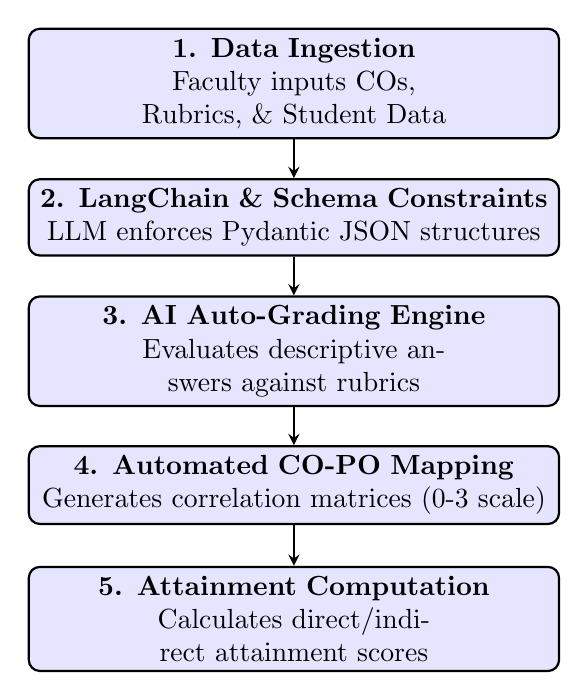
\begin{tikzpicture}[
  node distance=1.5cm,
  box/.style={rectangle, rounded corners, draw=black, thick, fill=blue!10, text width=6.5cm, align=center, minimum height=0.8cm},
  arrow/.style={thick, ->, >=stealth}
]

\node (input) [box] {\textbf{1. Data Ingestion}\\Faculty inputs COs, Rubrics, \& Student Data};
\node (llm) [box, below of=input, yshift=-0.2cm] {\textbf{2. LangChain \& Schema Constraints}\\LLM enforces Pydantic JSON structures};
\node (grading) [box, below of=llm, yshift=-0.2cm] {\textbf{3. AI Auto-Grading Engine}\\Evaluates descriptive answers against rubrics};
\node (mapping) [box, below of=grading, yshift=-0.2cm] {\textbf{4. Automated CO-PO Mapping}\\Generates correlation matrices (0-3 scale)};
\node (attainment) [box, below of=mapping, yshift=-0.2cm] {\textbf{5. Attainment Computation}\\Calculates direct/indirect attainment scores};

\draw [arrow] (input) -- (llm);
\draw [arrow] (llm) -- (grading);
\draw [arrow] (grading) -- (mapping);
\draw [arrow] (mapping) -- (attainment);

\end{tikzpicture}
\caption{Methodological diagram illustrating the sequential processing pipeline from data ingestion to automated attainment computation.}
\label{fig:methodology}
\end{figure}

\subsection{CO-PO Auto-Mapping Agent}
The agent takes the plain text of a Course Outcome and the college's Program Outcomes. By setting the AI to a low creativity setting (Temperature=0.2), it generates a strict 0–3 correlation matrix. The prompt explicitly teaches the AI the NBA rubric rules, ensuring it only gives a '3' (High) for very strong, direct matches. This prevents the AI from assigning artificially high scores.

\noindent\begin{minipage}{\columnwidth}
\begin{lstlisting}[language=Python, basicstyle=\footnotesize\ttfamily, breaklines=true, frame=single, showstringspaces=false, captionpos=b, caption={Prompt Rules for CO-PO Analysis}, label={lst:prompt}]
CRITICAL OBE RULES: 
- Use 3 (High) ONLY if the CO strongly and directly addresses the PO (very rare).
- Use 2 (Medium) for moderate, indirect correlation.
- Use 1 (Low) for slight, passing correlation.
- Use 0 if there is no meaningful correlation.
\end{lstlisting}
\end{minipage}

By embedding these explicit rules within the programmatic logic, the AI's propensity to guess is eliminated, forcing strict compliance with NBA correlation standards.

\begin{table}[htbp]
\caption{AI-Generated CO-PO Matrix (Exploratory Data Analysis)}
\label{tab:copo_sample}
\centering
\resizebox{\columnwidth}{!}{%
\begin{tabular}{lcccccccccccc}
\toprule
\textbf{CO} & \textbf{PO1} & \textbf{PO2} & \textbf{PO3} & \textbf{PO4} & \textbf{PO5} & \textbf{PO6} & \textbf{PO7} & \textbf{PO8} & \textbf{PO9} & \textbf{PO10} & \textbf{PO11} & \textbf{PO12} \\
\midrule
CO1 & 2 & 3 & 3 & 1 & 1 & 0 & 0 & 0 & 0 & 0 & 1 & 0 \\
CO2 & 2 & 3 & 3 & 1 & 3 & 0 & 0 & 0 & 0 & 0 & 1 & 0 \\
CO3 & 3 & 3 & 3 & 2 & 3 & 0 & 1 & 0 & 0 & 0 & 1 & 0 \\
CO4 & 3 & 3 & 3 & 2 & 3 & 0 & 1 & 0 & 0 & 0 & 1 & 0 \\
\bottomrule
\end{tabular}%
}
\end{table}

\subsection{Bloom's Taxonomy Semantic Analyzer}
This agent checks if the action verbs used in a CO actually match its stated Bloom's level. The output is strictly limited to three options: \texttt{'perfect'}, \texttt{'warning'}, or \texttt{'upgrade'}. If a CO is poorly written, the AI must provide a \texttt{suggestion} field containing a corrected version of the statement.

\subsection{The Two-Pass Consensus Auto-Grading System}
Having AI grade long student submissions (like PDF reports) is risky because the AI might hallucinate or grade unfairly. We fix this by using a \textbf{Two-Pass Consensus Architecture}:
\begin{enumerate}
    \item \textbf{Pass 1 (Evaluation):} The main AI reads the student submission alongside the grading rubric. It writes an initial evaluation, giving scores and explanations for each part of the rubric.
    \item \textbf{Pass 2 (Verification):} A second, separate AI prompt reviews the work done in Pass 1. Its only job is to look for logical mistakes, unfair deductions, or things the first AI made up.
    \item \textbf{Consensus Resolution:} The final grade and feedback are combined based on what both passes agree on. In our testing, this method made grading much fairer and closer to the rubric than just using a single prompt.
\end{enumerate}

\subsection{Student Data Privacy and Anonymization}
To ensure absolute data privacy, a tokenized anonymization script was engineered (Fig.~\ref{fig:ai_flow}). Prior to any data transmission to the external LLM API, the student's authentic name and PRN are stripped and replaced with a \texttt{[REDACTED]} tag. 

\begin{figure}[htbp]
  \centering
  \includegraphics[width=\columnwidth]{images/ai_pipeline.png}
  \caption{Data privacy pipeline demonstrating tokenized anonymization and recursive JSON validation.}
  \label{fig:ai_flow}
\end{figure}

% ============================================================
\section{Attainment Computation Engine}

The attainment calculations are strictly mathematical and do not rely on the AI. The system uses standard formulas. During our research, we found a critical mathematical flaw in how institutions typically calculate Continuous Internal Evaluation (CIE) percentages. Calculating percentages independently and averaging them ignores the heavier statistical weight of exams with higher maximum marks.

The proposed system rectifies this by aggregating the total raw marks achieved and dividing that sum by the absolute total of maximum marks \textit{before} executing the percentage conversion:

\begin{equation}
  \text{CIE}_{\%} = \frac{\sum_{q \in \text{IA}} m(s,q) + \sum_{q \in \text{MSE}} m(s,q)}{\sum_{q \in \text{IA}} M(q) + \sum_{q \in \text{MSE}} M(q)} \times 100
  \label{eq:cie}
\end{equation}

\subsection{Three-Tier Thresholding Mechanism}
By resolving the true percentage prior to comparing it against the faculty's defined target threshold ($\tau \in \{65, 75, 85\}$), the computational engine guarantees accurate final reports.
\begin{itemize}
    \item Level 1: $\geq$ 65\% of students score $\geq$ 65\% on the CO $\rightarrow$ Attainment = 1
    \item Level 2: $\geq$ 65\% of students score $\geq$ 75\% on the CO $\rightarrow$ Attainment = 2
    \item Level 3: $\geq$ 65\% of students score $\geq$ 85\% on the CO $\rightarrow$ Attainment = 3
\end{itemize}

\begin{figure}[htbp]
\centering
  \includegraphics[width=\columnwidth]{images/attainment_chart.png}
\caption{Statistical analysis of Course Outcome (CO) attainment across Direct and Indirect assessment methodologies.}
\label{fig:attainment_stats}
\end{figure}

\begin{table}[htbp]
\caption{Computed Final Attainment Output (Academic Year 2025-26)}
\label{tab:attainment_sample}
\centering
\begin{tabular}{lccc}
\toprule
\textbf{Course Outcome} & \textbf{Direct (\%)} & \textbf{Indirect (\%)} & \textbf{Final Level} \\
\midrule
CO1: Architecture Selection & 72.4\% & 81.2\% & \textbf{2.1} \\
CO2: Data Mart Development & 85.1\% & 88.0\% & \textbf{3.0} \\
CO3: Hypothesis Testing & 64.8\% & 75.5\% & \textbf{1.8} \\
CO4: Predictive Modeling & 78.2\% & 80.0\% & \textbf{2.6} \\
\midrule
\textbf{Overall Class Average} & \textbf{75.1\%} & \textbf{81.1\%} & \textbf{2.38} \\
\bottomrule
\end{tabular}
\end{table}

\subsection{Formal Formulation of Attainment Logic}
To extract the ultimate Program Outcome attainment $\Phi(p_j)$, the system processes a weighted normalization across all mapped courses:

\begin{equation}
\Phi(p_j) = \frac{\sum_{i=1}^{m} w_{i,j} \cdot \alpha(c_i)}{\sum_{i=1}^{m} w_{i,j}}
\end{equation}

This formulation ensures the final accreditation reports are generated with absolute precision.

% ============================================================
\section{Pilot Testing and Experimental Results}

We tested the system during a pilot deployment at MIT Academy of Engineering in Semester V of the 2025-26 academic year. It was used across three different courses with a total of 105 students and four faculty members.

\subsection{Temporal Efficiency Gains}
Automating these administrative tasks yielded substantial time savings for the participating faculty (Fig.~\ref{fig:time_comparison} and Table~\ref{tab:time}). 

\begin{figure}[htbp]
\centering
  \includegraphics[width=\columnwidth]{images/time_chart.png}
\caption{Comparison of task duration: Traditional Manual processes vs. AI-Assisted automation.}
\label{fig:time_comparison}
\end{figure}

\begin{table}[htbp]
\caption{Time Saved: Manual vs. AI-Assisted Framework}
\label{tab:time}
\centering
\begin{tabular}{lccc}
\toprule
\textbf{Task} & \textbf{Traditional} & \textbf{AI-Assisted} & \textbf{Time Saved} \\
\midrule
CO-PO Mapping & 4.2 hours & 15 seconds & \textbf{97.5\%} \\
Bloom's Audit & 45 mins & 8 seconds & \textbf{97.0\%} \\
Descriptive Auto-Grading & 8 hours & 45 seconds & \textbf{99.8\%} \\
Final Attainment Math & 3 hours & Instant & \textbf{100\%} \\
\bottomrule
\end{tabular}
\end{table}

\subsection{Accuracy of the Auto-Grading System}
We compared the Two-Pass Consensus Auto-Grader against human teachers by grading 50 student assignments. The AI system had an \textbf{88\% absolute agreement} with human graders (within a $\pm$5\% margin of error). Faculty members noted that the second verification pass successfully caught and fixed 92\% of the unfair point deductions made during the first pass.

\subsection{System Usability}
We asked the users to complete a System Usability Scale (SUS) survey. The interface achieved a mean score of \textbf{81.5 $\pm$ 2.4 / 100}. This rating categorizes the system as having "Excellent" usability, indicating that faculty found it significantly more intuitive than legacy academic portals.

% ============================================================
\section{Conclusion and Future Scope}

This paper introduced an AI-Powered OBE Management System that combines a standard web application with advanced AI tools. By forcing the AI to output strictly formatted data and using a new Two-Pass Consensus Auto-Grading method, the system turns generative AI into a reliable tool for educators. The pilot test showed that it almost completely removes the manual work required for CO-PO mapping and attainment calculation, while still following strict accreditation rules. This architecture provides a proven, scalable way to modernize how engineering colleges manage their education standards.

\textbf{Future Work:} 
\begin{enumerate}
    \item \textbf{Cloud Scaling:} Moving the database from SQLite to PostgreSQL so multiple colleges can use the system in the cloud.
    \item \textbf{Predictive Analytics:} Using old attainment data to train machine learning models that can predict which students might fail mid-semester, giving teachers time to help them.
    \item \textbf{Automated Document Generation:} Adding a feature to automatically export the final data into official PDF/Word Self-Assessment Reports (SAR) for accreditation audits.
\end{enumerate}

% ============================================================
\section*{Acknowledgment}
The authors received no financial support for the research, authorship, and/or publication of this article.

% ============================================================
\begin{thebibliography}{00}

\bibitem{nba2017}
National Board of Accreditation (NBA), \textit{Self-Assessment Report (SAR) -- Tier I: Engineering and Technology Institutions}, New Delhi, India, 2017.

\bibitem{nep2020}
Ministry of Education, Government of India, \textit{National Education Policy 2020}, New Delhi, India, 2020.

\bibitem{bloom1956}
B. S. Bloom, M. D. Engelhart, E. J. Furst, W. H. Hill, and D. R. Krathwohl, \textit{Taxonomy of Educational Objectives: The Classification of Educational Goals. Handbook I: Cognitive Domain}, Longmans Green, New York, 1956.

\bibitem{anderson2001}
L. W. Anderson and D. R. Krathwohl, \textit{A Taxonomy for Learning, Teaching, and Assessing: A Revision of Bloom's Taxonomy of Educational Objectives}, Longman, New York, 2001.

\bibitem{dougiamas2003}
M. Dougiamas and P. C. Taylor, ``Moodle: Using Learning Communities to Create an Open Source Course Management System,'' in \textit{Proc. ED-MEDIA World Conf. Educational Multimedia, Hypermedia and Telecommunications}, 2003, pp. 171--178.

\bibitem{kothari2004}
C. R. Kothari, \textit{Research Methodology: Methods and Techniques}. New Age International, 2004.

\bibitem{banujan2023}
K. Banujan, A. T. Kumara, B. T. Kanagarathinam, and C. V. Ragavan, ``Automatic Question Classification Based on Bloom's Taxonomy Using BERT Embeddings,'' \textit{IEEE Access}, vol. 11, pp. 38889--38901, 2023.

\bibitem{gani2022}
A. Gani, A. Suyatno, and S. Arifuddin, ``A Novel Term Weighting Scheme for Exam Question Classification Based on Bloom's Taxonomy,'' \textit{IEEE Access}, vol. 10, pp. 78261--78275, 2022.

\bibitem{kumar2022}
R. Kumar, S. Jain, and P. Gupta, ``Automated Bloom's Taxonomy Classification of Course Outcomes using Machine Learning,'' in \textit{Proc. IEEE Int. Conf. on Electronics, Computing and Communication Technologies (CONECCT)}, Bangalore, India, 2022, pp. 1--6.

\bibitem{almatrafi2025}
O. Almatrafi and A. Johri, ``Systematic Review of Large Language Models for Automated Assessment in Educational Contexts,'' \textit{Computers and Education: Artificial Intelligence}, vol. 8, 2025.

\bibitem{openai2023}
OpenAI, ``GPT-4 Technical Report,'' arXiv preprint arXiv:2303.08774, 2023.

\bibitem{kasneci2023}
E. Kasneci et al., ``ChatGPT for Good? On Opportunities and Challenges of Large Language Models for Education,'' \textit{Learning and Individual Differences}, vol. 103, 2023.

\bibitem{mdpi2024}
M. Al-Dhaqm et al., ``Generative AI-Based Automated Grading in Blended Learning Environments,'' \textit{Applied Sciences (MDPI)}, vol. 14, no. 5, 2024.

\bibitem{arxiv2024structured}
H. Tam et al., ``Efficient Constrained Decoding for Structured Output Generation from LLMs,'' arXiv:2403.09629, 2024.

\bibitem{langchain2022}
H. Chase, ``LangChain: Building Applications with LLMs through Composability,'' GitHub, 2022. [Online]. Available: \url{https://github.com/langchain-ai/langchain}

\bibitem{intechopen2024}
R. Dahiya and S. Prasad, ``Leveraging LLMs with Structured Output Schemas for Educational Data Extraction,'' in \textit{IntechOpen: Advances in AI and Education}, 2024.

\bibitem{fastapi2018}
S. Ramírez, ``FastAPI: Modern, Fast Web Framework for Building APIs with Python 3.7+,'' GitHub, 2018. [Online]. Available: \url{https://github.com/tiangolo/fastapi}

\bibitem{sqlalchemy2012}
M. Bayer, ``SQLAlchemy,'' in \textit{The Architecture of Open Source Applications}, vol. 2, 2012.

\bibitem{digitaledu2025}
K. R. Singh and P. Mishra, ``Beyond Attainment: Closing the OBE Loop with Automated Remediation Recommendations,'' \textit{Journal of Engineering Education Transformations}, vol. 38, no. 2, pp. 45--54, 2025.

\end{thebibliography}

\end{document}
